\subsection{Sabath (SBI-FAIR)}
{{\footnotesize
\noindent Sabath is a metadata framework from the SBI-FAIR group (UTK, Argonne, Virginia) facilitating
FAIR-compliant benchmarking and surrogate execution logging across HPC systems .


\begin{description}[labelwidth=4cm, labelsep=1em, leftmargin=4cm, itemsep=0.1em, parsep=0em]
  \item[date:] 2021-09-27
  \item[version:] v1.0
  \item[last\_updated:] 2023-07
  \item[expired:] unknown
  \item[valid:] yes
  \item[valid\_date:] 2021-09-27
  \item[url:] \href{https://sbi-fair.github.io/docs/software/sabath/}{https://sbi-fair.github.io/docs/software/sabath/}
  \item[doi:] unknown
  \item[domain:] Systems; Metadata
  \item[focus:] FAIR metadata framework for ML-driven surrogate workflows in HPC systems
  \item[keywords:]
    - meta-benchmark
    - metadata
    - HPC
    - surrogate modeling
  \item[licensing:] BSD 3-Clause License
  \item[task\_types:]
    - Systems benchmarking
  \item[ai\_capability\_measured:]
    - Metadata tracking
    - reproducible HPC workflows
  \item[metrics:]
    - Metadata completeness
    - FAIR compliance
  \item[models:]
    - NA
  \item[ml\_motif:]
    - Systems
  \item[type:] Platform
  \item[ml\_task:]
    - NA
  \item[solutions:] 0
  \item[notes:] Developed by PI Piotr Luszczek at UTK; integrates with MiniWeatherML, AutoPhaseNN, Cosmoflow, etc. 

  \item[contact.name:] Piotr Luszczek
  \item[contact.email:] luszczek@utk.edu
  \item[results.links.name:] ChatGPT LLM
  \item[fair.reproducible:] Yes
  \item[fair.benchmark\_ready:] N/A
  \item[id:] sabath\_sbi-fair
  \item[Citations:] \cite{luszczek2021sabath}
\end{description}

{\bf Ratings:} ~ \\

\begin{tabular}{p{0.15\textwidth} p{0.07\textwidth} p{0.7\textwidth}}
\hline
Rating & Value & Reason \\
\hline
dataset & 4 & Datasets used in surrogate benchmarks are publicly available, well-structured, and
FAIR-aligned, but not independently hosted by Sabath itself.
 \\
documentation & 3 & Basic instructions and code are provided on GitHub, but more detailed walkthroughs,
use-case examples, or tutorials are limited.
 \\
metrics & 4 & Emphasizes metadata completeness and FAIR compliance. Metrics are clear and well-matched
to its metadata-focused benchmarking context.
 \\
reference\_solution & 3 & Includes integration with multiple surrogate benchmarks and models, though not all are
fully documented or packaged as standardized reference solutions.
 \\
software & 4 & Actively maintained GitHub repository (https://github.com/icl-utk-edu/slip/tree/sabath)
with BSD-licensed tooling for FAIR metadata capture; integrates with existing surrogate
modeling benchmarks.
 \\
specification & 4 & FAIR metadata structure and logging goals are clearly described. Input/output definitions
are implied through integrations (e.g., MiniWeatherML), though not always formalized.
 \\
\hline
\end{tabular}

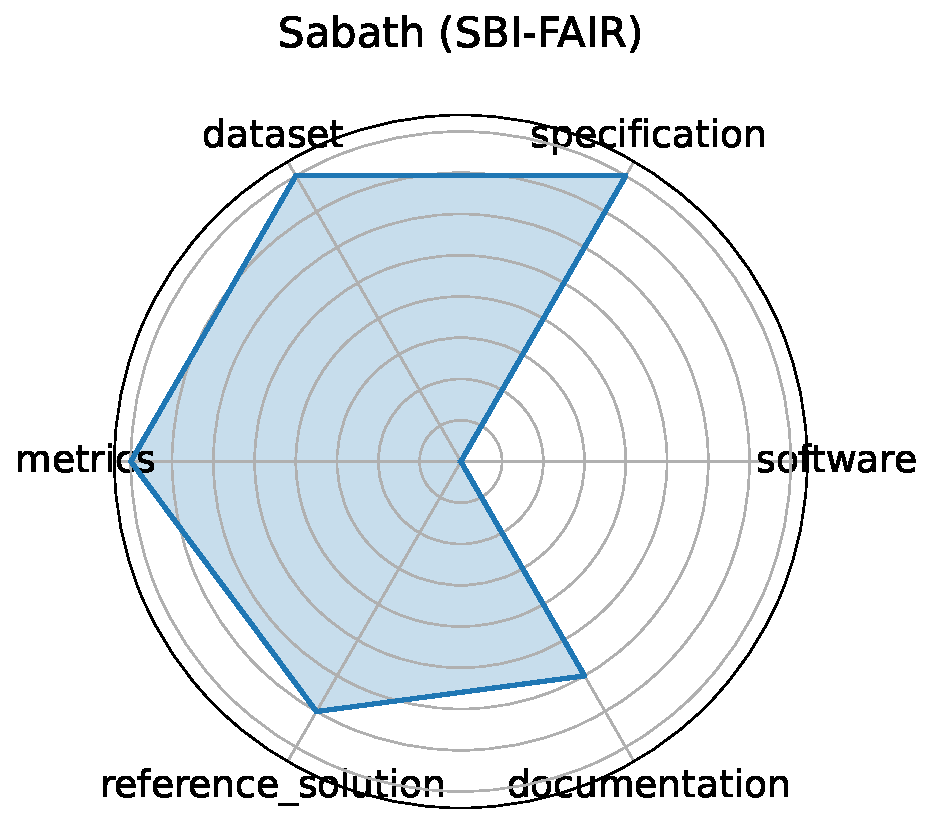
\includegraphics[width=0.2\textwidth]{sabath_sbi-fair_radar.pdf}
}}
\clearpage